 \areaset[0cm]{14cm}{28cm} 
\section{The urinary system}
\subsection{Maintenance of the composition of body fluids}

\Kommentar{Intro: why we need the urinary system - ref to the BB-scheme "`metabolism"' --> 10 min}{}{1.4cm}{}

Read \ding{229} Starr (9ed) chapter 37.1 (p.650-651) and answer the following questions: \marginline{\textbf{hint}: \textit{search the key terms given in the question and read your text from there.}}
	\begin{enumerate}[itemsep=1.5em, leftmargin=*]
	\item  What relates proteins to urea and to urine?
		\Loesung{	proteins (and other nitrogen containing molecules) eventually need to be broken down\\
			the breakdown product of proteins is \emph{urea} in mammals \\
			urea is water soluble and is excreted with some water as \emph{urine}.
			}{3cm}
	\item Why can birds or reptiles do it for a longer time than mammals without drinking?
		\Loesung{ Birds and reptiles form uric acid\\
			 excretion of uric acid requires 20 to 30 times less water to excrete than urea
			}{3cm}
	\item What are the organs called that adjust salt and water concentrations in body fluids? \\
		\ldots in reptiles: \gap{...kidneys ...}\\
		\ldots in earth worms: \gap{...nephridia (plural) / nephridium (sing.) ...}\\
		\ldots in mammals: \gap{...kidneys ...}\\
		\ldots in insects: \gap{...Malpighian tubules ...}\\
		\ldots in fish: \gap{...kidneys ...}\\
	\item Use your text (Starr, 37.1) to comment figures \ref{fig:OsmoregulationMeer} and \ref{fig:OsmoregulationSuessw}
		
	\end{enumerate}
	
	\Ersatz{
			    \begin{figure}[htbp]
			    \begin{minipage}{0.46\textwidth}
			     \centering
			      \includegraphics[width=1\textwidth]{../images/OsmoregulationMeer_Cornelsen.png}
			      \caption [Osmoregulation Meerfisch aus Cornelsen SII]{Osmotic regulation in salt water fish. \textit{Explain this process:} \textcolor{red}{Salt water fish risks to loose water due to osmosis; active excretion of excess salt is necessary, accompanied by formation of only small amounts of urine}}  \label{fig:OsmoregulationMeer}
			    \end{minipage}\hfill
			    \begin{minipage}{0.48\textwidth}
			     \centering
			      \includegraphics[width=1\textwidth]{../images/OsmoregulationSuessw_Cornelsen.png}
			      \caption[Osmoregulation bei Süsswasserfischen aus Cornelsen SII]{Osmotic regulation in fresh water fish. \textit{Explain this process:} \textcolor{red}{Fresh water fish risks to burst due to osmotic water uptake; formation of very high amounts of urine, accompanied by active uptake of salts from water}}  \label{fig:OsmoregulationSuessw}
			    \end{minipage}
 				 \end{figure}
		}{%
			    \begin{figure}[htbp]
			    \begin{minipage}{0.46\textwidth}
			     \centering
			      \includegraphics[width=1\textwidth]{../images/OsmoregulationMeer_Cornelsen-sw.png}
			      \caption [Osmoregulation Meerfisch aus Cornelsen SII]{Osmotic regulation in salt water fish. \textit{Explain this process:} \dotfill \\ \ldots \dotfill \\ \ldots \dotfill  \\ \ldots \dotfill }  \label{fig:OsmoregulationMeer}
			    \end{minipage}\hfill
			    \begin{minipage}{0.48\textwidth}
			     \centering
			      \includegraphics[width=1\textwidth]{../images/OsmoregulationSuessw_Cornelsen-sw.png}
			      \caption[Osmoregulation bei Süsswasserfischen aus Cornelsen SII]{Osmotic regulation in fresh water fish. \textit{Explain this process:} \dotfill \\ \ldots \dotfill \\ \ldots \dotfill  \\ \ldots \dotfill }  \label{fig:OsmoregulationSuessw}
			    \end{minipage}
 				 \end{figure}
			}%



 
\subsection{The human urinary system}
Read \ding{229} Starr chapter 37.2 and use the following questions and figures to check your understanding

		\begin{figure}[htp]
		  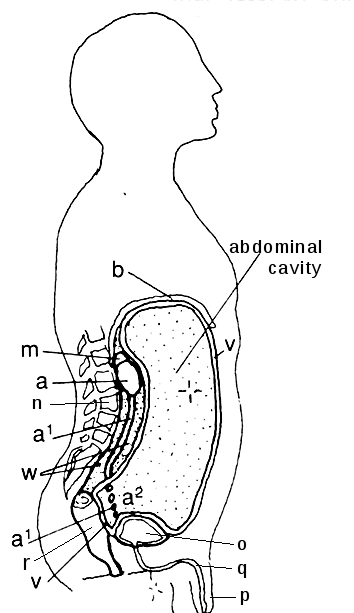
\includegraphics[width=0.4\textwidth]{../images/AnatomieMalatlas109-2_sw_v3.png}
		  \caption[Sagital cut of the trunk]{This is a sagital cut of a human body. Use table \ref{tab:UrinarySystemSagital} to complete the legend!}
		  \label{fig:UrinarySystemSagital}
		%\setfloatalignment{b}
		\end{figure}

	\hspace{-2cm}
	\begin{minipage}{14cm}
	\setlength{\extrarowheight}{4pt}	
	\captionof{table}[VERZEICHNIS]{Legend for figure \ref{fig:UrinarySystemSagital} - use Starr complete the terms. }
	  \vspace{12pt}  \hspace{0cm}
	       \begin{tabularx}{14cm}[]{p{1.5cm} p{4.5cm} p{1.5cm} p{4.5cm}} 
	\toprule
	\#  & anatomical term & \#  & anatomical term  file\\\midrule
	 a  & \gap{kidney} & o   & \gap{bladder} \\
	 a1  & \gap{ureter}  & p  & \gap{urethra} \\
	 a2  & \gap{ureter}  & q  & \gap{penis} \\
	 b  & \gap{diaphragm}  & r  & \gap{rectum} \\
	 m  & \gap{adrenal gland}  & v  & \gap{peritoneum} \\
	 n   & \gap{back bone}  & w  & retroperitoneum \\
	\bottomrule
	\end{tabularx}%
	  \label{tab:UrinarySystemSagital}%
	\end{minipage}


	\hspace{-1cm}
	\begin{minipage}[b]{9cm}
		\centering {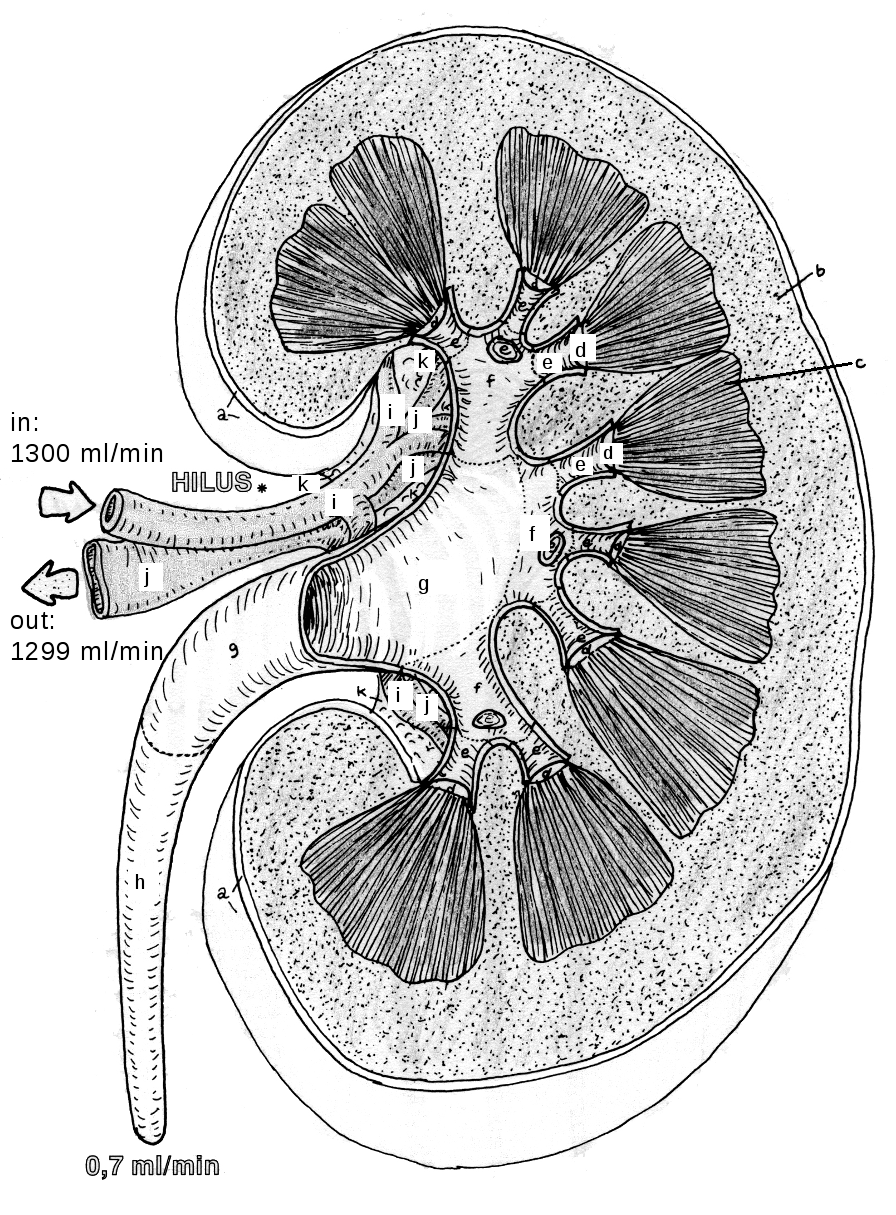
\includegraphics[width=1\linewidth]{../images/AnatomieMalatlas110_b_sw_v1.png}}   \captionof{figure}[Niere koronal, AnatomieMalatlas110b]{Cross section through the left kidney. Use table \ref{tab:KidneyCrossEntire} to complete the legend!} 	\label{fig:KidneyCrossEntire}
	\vspace{0.6pt}
	\end{minipage}
	\hspace{0.5cm}
	\begin{minipage}[b]{7cm}
	\centering {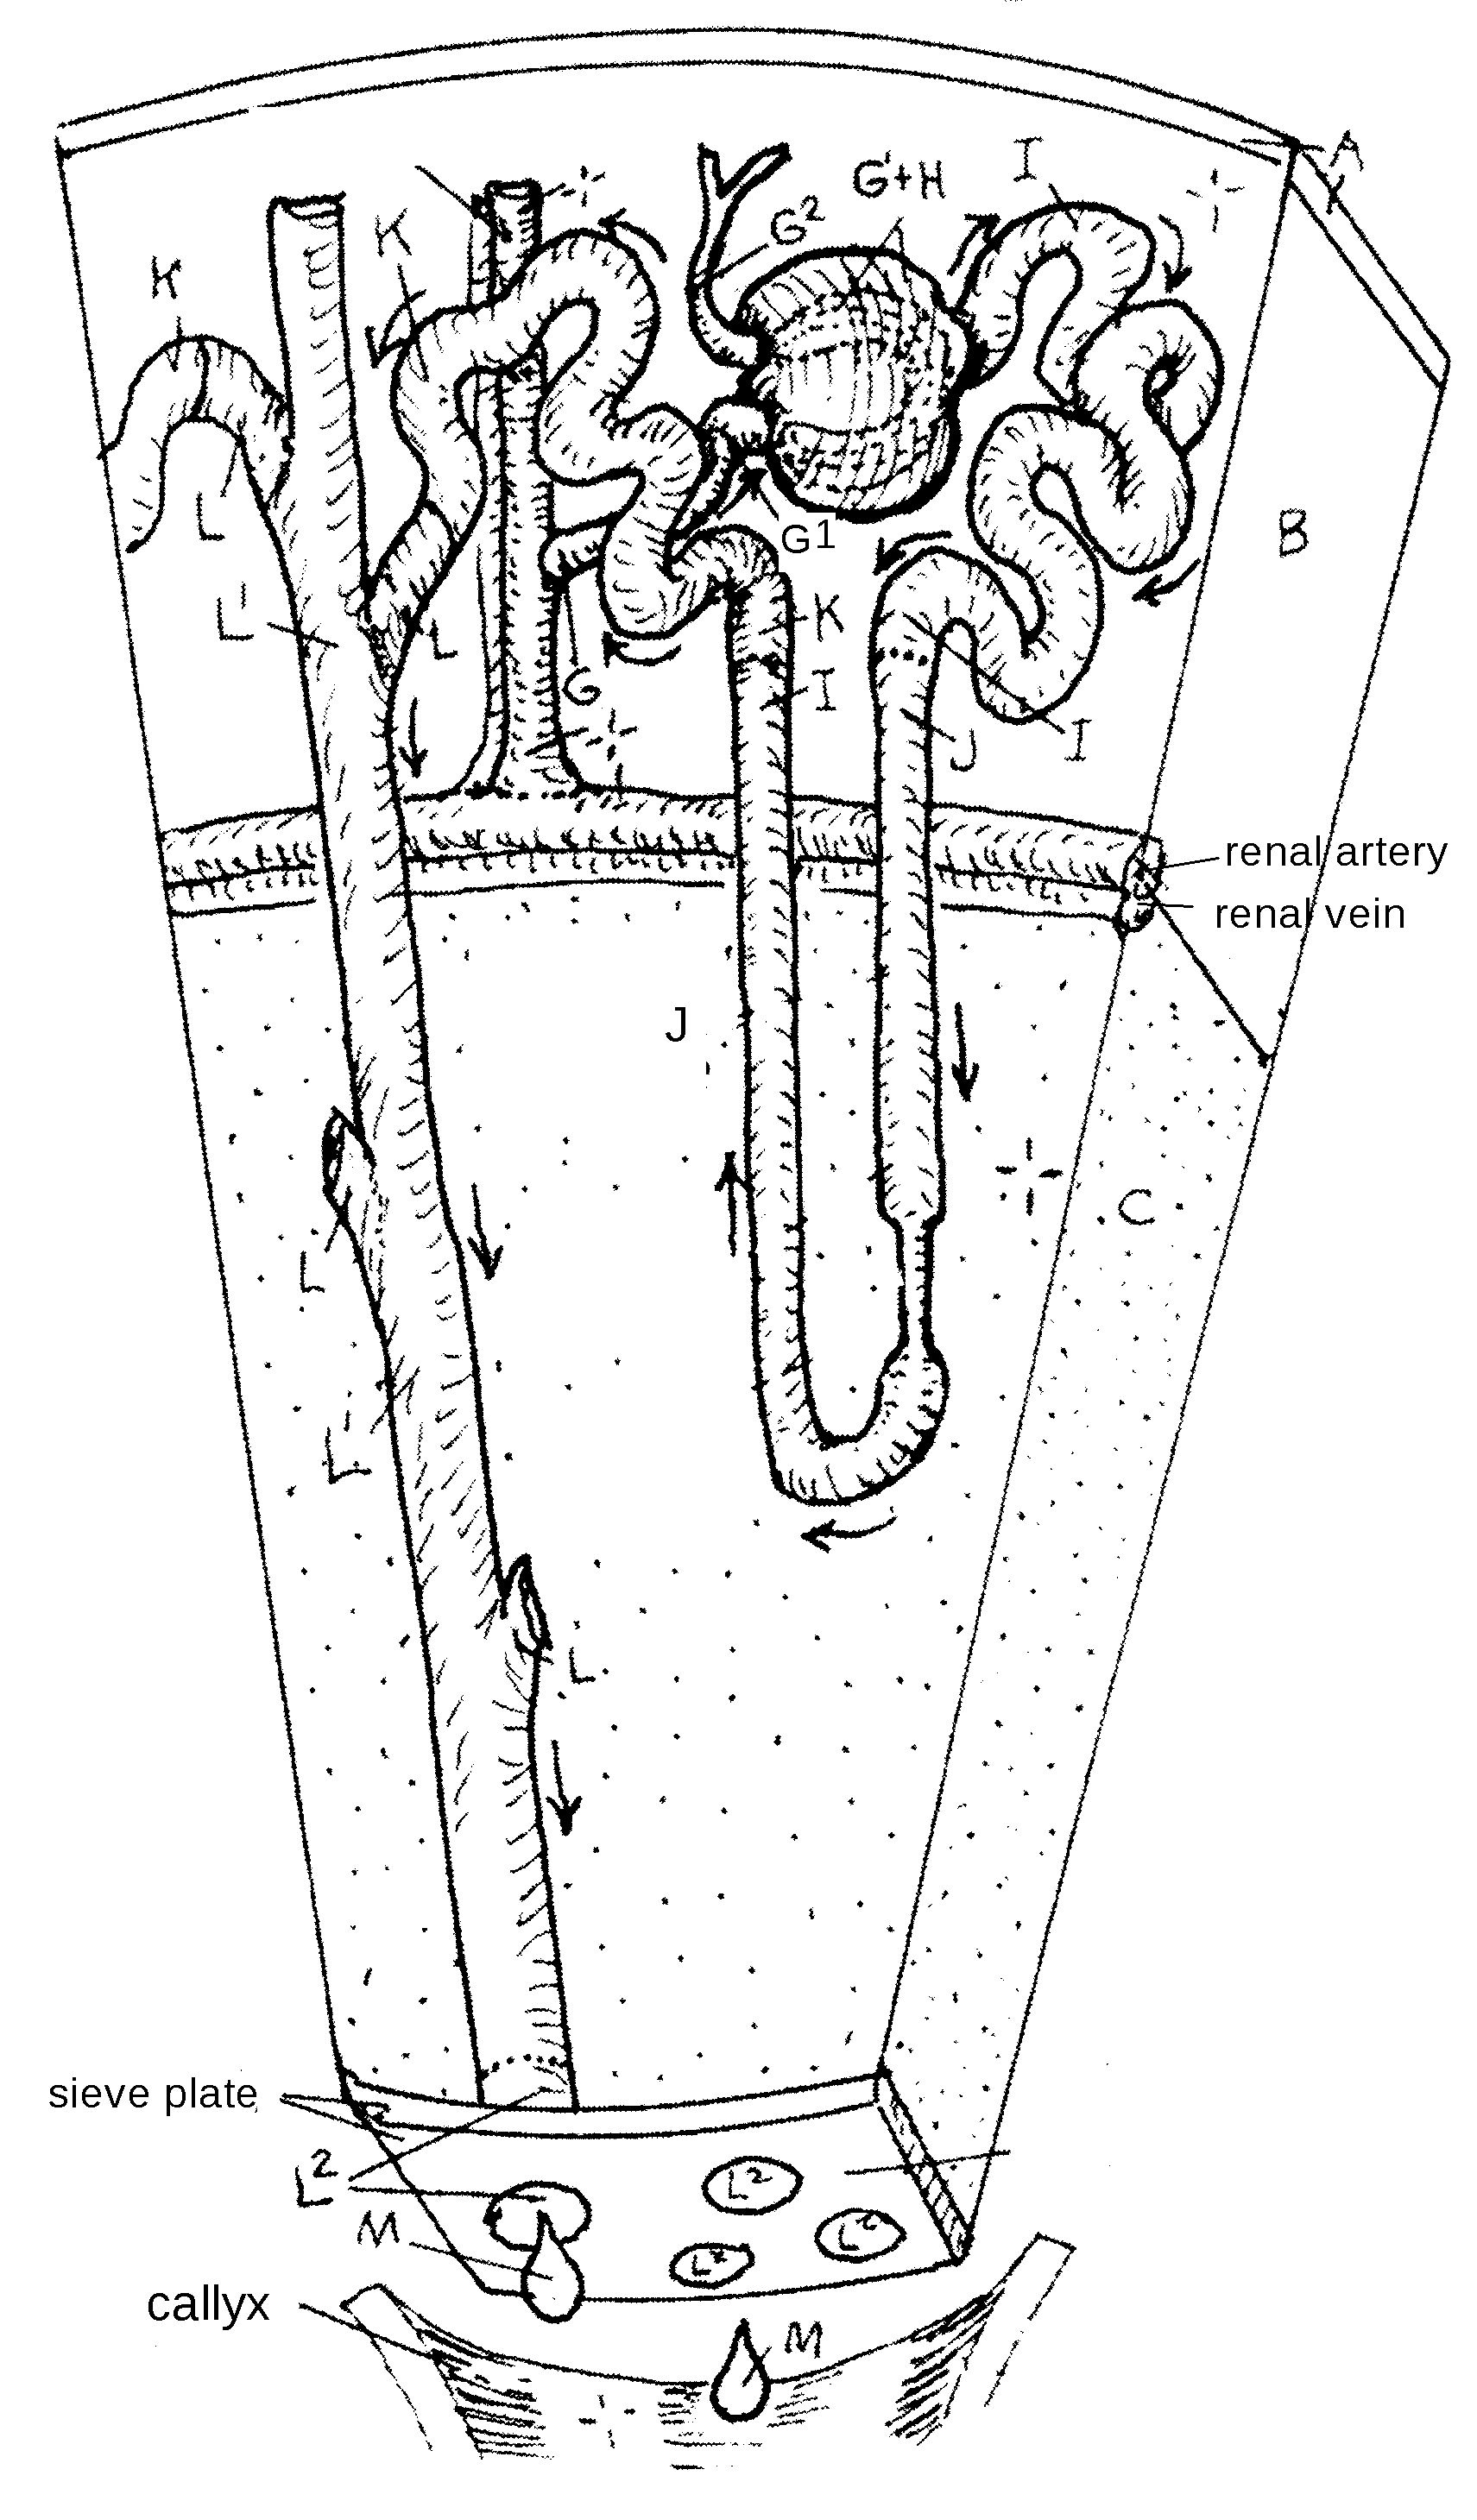
\includegraphics[width=1\linewidth]{../images/AnatMalAtl2_299-3_v1.png}}   \captionof{figure}[Nephron, AnatMalAtl2-299-3]{Enlarged view of renal cortex and medulla. Use table \ref{tab:KidneyCortexMedulla} to complete the legend!}  	\label{fig:KidneyCortexMedulla}
	\vspace{2pt}
	\end{minipage}
	
\enlargethispage{1.2cm}
	
	\marginline{Use colour pencils (red, blue) and \textbf{add} the \emph{peritubular capillaries} in figure \ref{fig:KidneyCortexMedulla}!}
	
		\hspace{-1cm}
	\begin{minipage}{14cm}
	\setlength{\extrarowheight}{2pt}	
	\captionof{table}[VERZEICHNIS]{Legend for figure \ref{fig:KidneyCrossEntire} - use Starr complete the terms. }
	  \vspace{12pt}  \hspace{0cm}
	       \begin{tabularx}{14cm}[]{p{1.5cm} p{4.5cm} p{1.5cm} p{4.5cm}} 
	\toprule
	\#  & anatomical term & \#  & anatomical term  \\\midrule
	 a  & \gap{renal capsule} & g   & \gap{renal pelvis} \\
	 b  & \gap{renal cortex}  & h  & \gap{ureter} \\
	  c & \gap{renal medulla}  & i  & \gap{renal artery} \\
	 d & apex of the pyramid  &  j & \gap{renal vein} \\
	 e & small callyx  &  k & -- \\
	  f  & large callyx  &   &  \\
	\bottomrule
	\end{tabularx}%
	  \label{tab:KidneyCrossEntire}%
	\end{minipage}
			\hspace{-1cm}
	\begin{minipage}{14cm}
	\setlength{\extrarowheight}{2pt}	
	\captionof{table}[VERZEICHNIS]{Legend for figure \ref{fig:KidneyCortexMedulla} - use Starr complete the terms. }
	  \vspace{12pt}  \hspace{0cm}
	       \begin{tabularx}{14cm}[]{p{1.5cm} p{4.5cm} p{1.5cm} p{4.5cm}} 
	\toprule
	\#  & anatomical term & \#  & anatomical term  \\\midrule
	  B & \gap{renal cortex} & I & \gap{proximal tubule}\\
	  C & \gap{renal medulla} & J & \gap{loop of Henle}\\
	  G & \textbf{renal artery } &  K  & \gap{distal tubule } \\
	  G1 & \gap{afferent arteriole }  & L   & \gap{collecting tubule} \\
	  G2 & \gap{efferent arteriole }  &   L2 & \gap{opening of tubule } \\
	  G+H & \gap{glomerulus (G) in Bowman capsule (H)} a  &  M & \gap{urin } \\
	\bottomrule
	\end{tabularx}%
	  \label{tab:KidneyCortexMedulla}%
	\end{minipage}
	
	
	 \areaset[0cm]{11.5cm}{27.4cm}  
	 
\subsection{Urine formation}
Read \ding{229} Starr chapter 37.3 and use the following figures and questions to deepen your knowledge!

\hspace{-3cm}
\begin{minipage}{15cm}
	 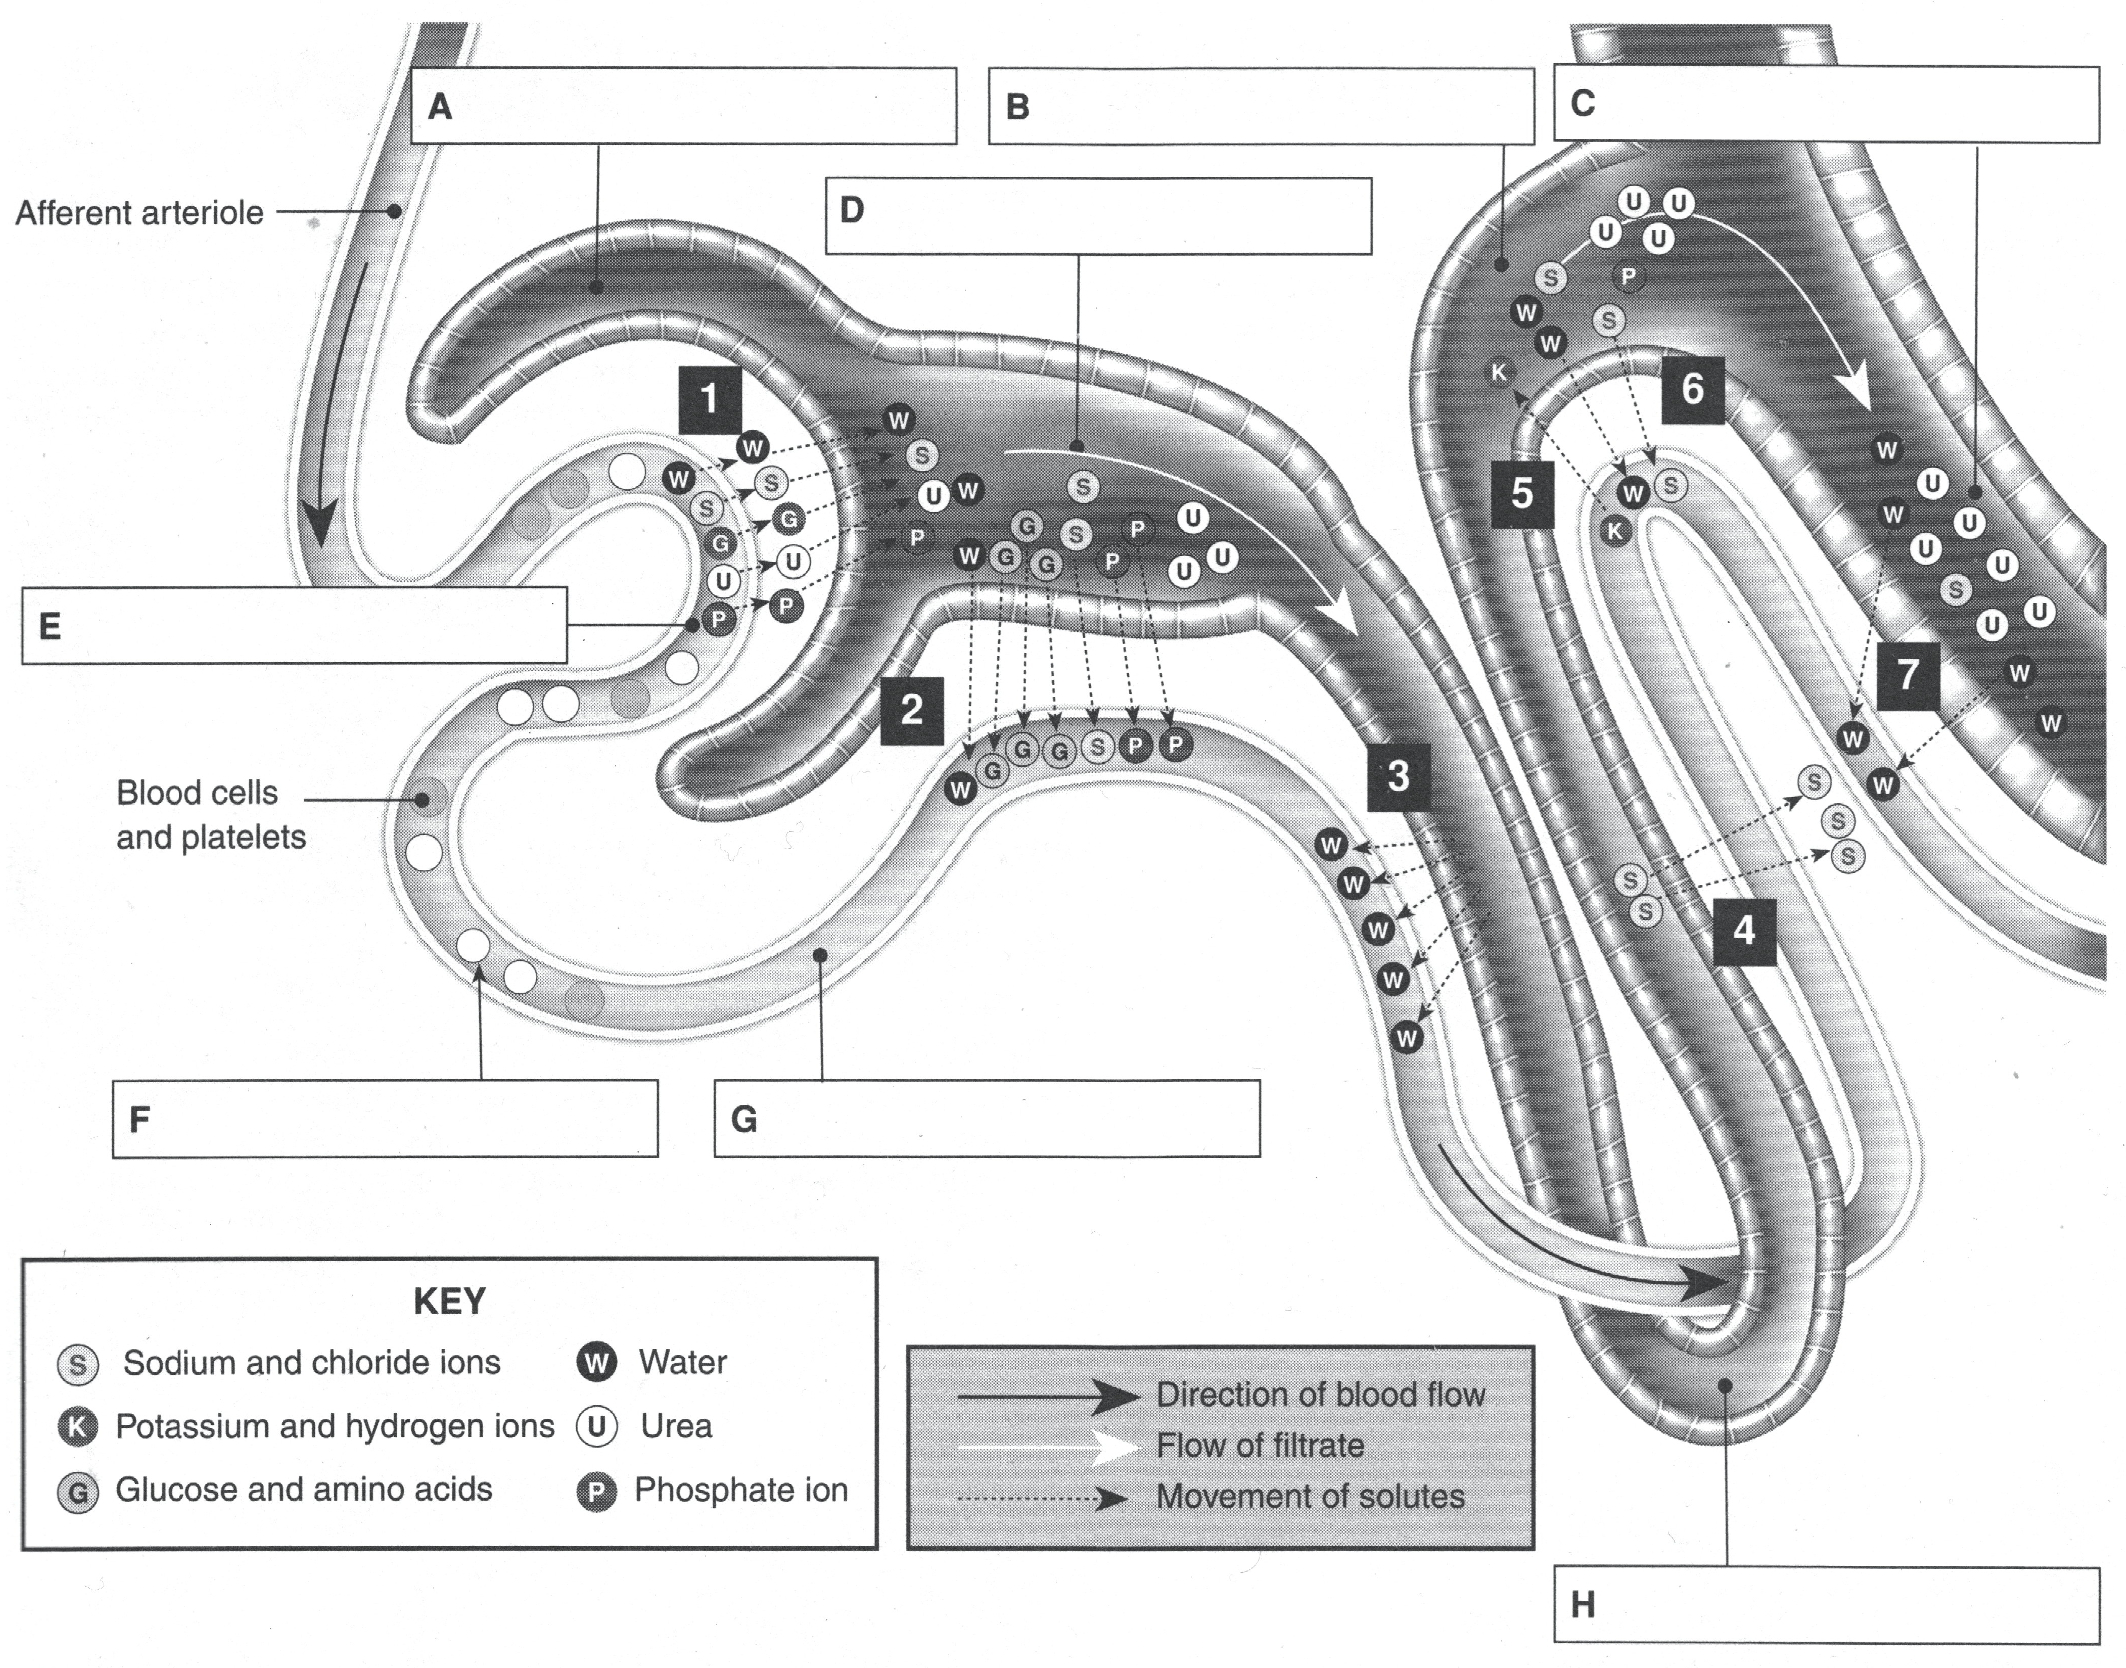
\includegraphics[width=1\textwidth]{../images/biozone-human-0202_v2.jpg}
		  \captionof{figure}[Urine foramtion overview biozone human p.222]{The diagram above presents an overview of the structures and processes involved in the formation of urine in the kidney. The structures involved are labelled with letters (A-H), while the major processes are identified with numbers (1-7).}
		  \label{fig:UrineFormationBiozone}
\end{minipage}
\begin{enumerate}[resume, leftmargin=*]
\item  Using the word list provided below, identify each of the structures marked with a letter (A - H) in figure \ref{fig:UrineFormationBiozone}. Write the name of the structure in the space provided on the diagram. 

	\emph{\gap{B} distal convoluted tubule; \gap{G} efferent arteriole; \gap{E} glomerulus; \gap{A} Bowman's capsule; \gap{D} proximal convoluted tubule; \gap{H} loop of Henle; \gap{F} large blood proteins; \gap{C} collecting duct }
	
\item Match each of the processes (identified on the diagram with numbers 1-7) to the correct summary of the process provided below. Write the process number next to the appropriate sentence. 
 \gap{ 4 }   Active transport of seit ( \ce{Na+} and  \ce{Cl-}) from the ascending Iimb of the loop of Henle. 
 \gap{ 1 }   Filtration through the membranes of the glornerulus. Glucose, water, and ions pass through. 
 \gap{ 2 }   Reabsorption of glucose and ions by active transport. Water follows by diffusion. 
 \gap{ 3 }   Reabsorption of water by osmosis from the descending limb of the loop of Henle. 
 \gap{ 5 }   Active secretion (into the filtrate) of  \ce{H+} and  \ce{K+}(  \ce{NH3} also diffuses into the filtrate). 
 \gap{ 7 }  Concentration of the urine by osmotic withdrawal of water from the flitrate. 
 \gap{ 6 }   Reabsorption of  \ce{Na+} and  \ce{Cl-} by active transport and water by osmosis. 

% \item There is marked gradient in salt concentration in the extracellular fluid of the medulla, produced by the transport of salt out of the filtrate. Explain the purpose of this salt gradient: 
\end{enumerate}

	 \areaset[0cm]{13cm}{27.4cm}  

\begin{landscape}

\subsubsection{Osmosis drives reabsorption}
\hspace{4 em} 
	
	\begin{minipage}[p]{20cm}
		\centering {\includegraphics[width=1\textwidth]{../images/PhysiolMalatl_059-A-small_Nieren.png}}   \captionof{figure}[PhysiolMalatl 059]{Filtration is driven by blood pressure; reabsorption is driven by osmosis: carefully explain these processes shown in this figure!}  	\label{fig:Filtration}
% 	\vspace{2pt}
	\end{minipage}
 
\end{landscape}

	 \areaset[0cm]{11.5cm}{27.4cm}  
	 
 \subsubsection{Crosscurrents maintain a salt concentration gradient}
 This issue is not covered in Starr. It's all about the \emph{increasing solute concentration in interstitial fluid} shown in Starr's figure 37.7
 
%  \Ersatz{
		    \begin{figure}[htbp]
		    \begin{minipage}{0.4\textwidth}
		     \centering
		      \includegraphics[width=1\textwidth]{../images/Gegenstromprinzip_Silbernagl-2.jpg}
		      \caption[Gegenstromprinzip aus Silbernagl]{Crosscurrent in a heating system}  	\label{fig:GegenstromWaermetauscher}
		    \end{minipage}\hfill
		    \begin{minipage}{0.4\textwidth}
		     \centering
		      \includegraphics[width=1\textwidth]{../images/Gegenstromprinzip_Silbernagl-3.jpg}
		      \caption[Gegenstrom-Vogel aus Silbernagl]{Crosscurrent keep bird's feet warm.}  	\label{fig:Flamingo}
		    \end{minipage}
			 \end{figure}
% 		}{
% 		   \piccaptionoutside
%  		\piccaption[Abb. zu Wärmetauscher selber zeichnen]{ \label{fig:BLA} Selber einzeichnen: "`Gegenstrom in einem Wärmetauscher"'}  	\label{fig:GegenstromWaermetauscher}
% 		\parpic(6.5cm,6cm)[f][l]{}
% 		   \piccaptionoutside
%  		\piccaption[Gegenstrom-Vogel aus Silbernagl]{ \label{fig:Flamingo} Vogel auf dem Eis - z.B. ein Flamingo}
% 		\parpic[r]{\includegraphics[width=6cm]{../images/Gegenstromprinzip_Silbernagl-3_sw.png}}	\picskip{0}
% 		}
 
 \vspace{2cm}
 	\begin{minipage}[htbp]{1\columnwidth}
	 {\includegraphics[width=1\linewidth]{../images/thews_p346-v1_sw.png}}   \captionof{figure}[Schema zum Aufbau des Konz-Gradienten; aus Thews]{Osmotic gradient in the renal medulla - all figures in mol per litre. The higher the figure, the more salt is dissolved in the interstitium, the space between the cells in the renal medulla.}  	\label{fig:KonzVerhaeltnis}
	\vspace{2pt}
	\end{minipage}
